\documentclass{egpubl}

% --- for  Annual CONFERENCE
% \ConferenceSubmission % uncomment for Conference submission
% \ConferencePaper      % uncomment for (final) Conference Paper
% \STAR                 % uncomment for STAR contribution
% \Tutorial             % uncomment for Tutorial contribution
% \ShortPresentation    % uncomment for (final) Short Conference Presentation
%
% --- for  CGF Journal
% \JournalSubmission    % uncomment for submission to Computer Graphics Forum
% \JournalPaper         % uncomment for final version of Journal Paper
%
% --- for  EG Workshop Proceedings
% \WsSubmission    % uncomment for submission to EG Workshop
 \WsPaper         % uncomment for final version of EG Workshop contribution
%
 \electronicVersion % can be used both for the printed and electronic version

% !! *please* don't change anything above
% !! unless you REALLY know what you are doing
% ------------------------------------------------------------------------

% for including postscript figures
% mind: package option 'draft' will replace PS figure by a filename within a frame
\ifpdf \usepackage[pdftex]{graphicx} \pdfcompresslevel=9
\else \usepackage[dvips]{graphicx} \fi

\PrintedOrElectronic

% prepare for electronic version of your document
\usepackage{t1enc,dfadobe}
\usepackage[utf8]{inputenc}

\usepackage[french,english]{babel}

\usepackage{amsmath}
\usepackage{amsfonts}
\usepackage{amssymb}

\usepackage{enumerate}
\usepackage{caption}
\usepackage{subcaption}
\usepackage{listings}

% Fonts packages (if needed)
%\usepackage[nott,fullsumlimits]{kpfonts}
%\usepackage{lmodern}

\usepackage{egweblnk}
\usepackage{cite}

% ---------------------------------------------------------------------
\title[ACA: The ``Smooth'' Challenge]{Advanced Computer Architecture: The ``Smooth'' Challenge}

\author[R. Brault \& A. Camus]{Romain Brault and Alexandre Camus}



% ------------------------------------------------------------------------
\begin{document}


% % listings options
\lstset{
basicstyle=\ttfamily,
keywordstyle=\color{blue},
identifierstyle=,
commentstyle=\color[rgb]{.2,.4,.5},
stringstyle=\ttfamily\color{gray},
language=C++}

% \teaser{
%  \includegraphics[scale=0.3&]{Imperial__4_colour_process.jpg}
%  \centering
%   \caption{New EG Logo}
% \label{fig:teaser}
% }

\maketitle

\begin{abstract}
   The ABSTRACT is to be in fully-justified italicized text, 
   between two horizontal lines,
   in one-column format, 
   below the author and affiliation information. 
   Use the word ``Abstract'' as the title, in 9-point Times, boldface type, 
   left-aligned to the text, initially capitalized. 
   The abstract is to be in 9-point, single-spaced type.
   The abstract may be up to 3 inches (7.62 cm) long. \\
   Leave one blank line after the abstract, 
   then add the subject categories according to the ACM Classification Index 
   (see http://www.acm.org/class/1998/).

\end{abstract}


%\tableofcontents


%-------------------------------------------------------------------------
\section{Introduction}

%% TODO

\subsection{Hardware Considerations}

The chosen hardware is not one of the machine from the Lab. They do not have any interesting GPUs. But one of our laptops is very powerful with an interesting GPU. This is the chosen one.

The table \ref{CPUspec} contains the details of this hardware.
\begin{table}[h]
\centering
\begin{tabular}{|l|r|}
\hline
Model Name & Intel Core i7 CPU Q720 \\
\hline
Clock Speed & 1.597 GHz \\
\hline
Max Turbo Frequency & 2.8 GHz \\
\hline
Cache size & 6144 KB \\
\hline
CPU cores & 4 \\
\hline
CPU Threads & 8 \\
\hline
Integrated GPU & No \\
\hline
Memory Channels & 2 \\
\hline
Max Memory Bandwith & 21 GB/s \\
\hline
\end{tabular}
\caption{CPU Specifications}
\label{CPUspec}
\end{table}

The GPU specifications are shown in the table \ref{GPUspecs}.

\begin{table}[h]
\centering
\begin{tabular}{|l|r|}
\hline
Model Name & NVIDIA GeForce GTX 260M \\
\hline
Clock Speed & 1.375 GHz \\
\hline
Multiprocessors & 14 \\
\hline
Global CUDA cores & 112 \\
\hline
Allocated Memory & 1 GB \\
\hline
Memory Clock Speed & 950 MHz \\
\hline
\end{tabular}
\caption{GPU Specifications}
\label{GPUspecs}
\end{table}

To summarize, the figure \ref{topo} gives a quick overview of the hardware topology. The GPU is connected on the PCI port \verb+10de:0618+.

\begin{figure}[h]
\centering
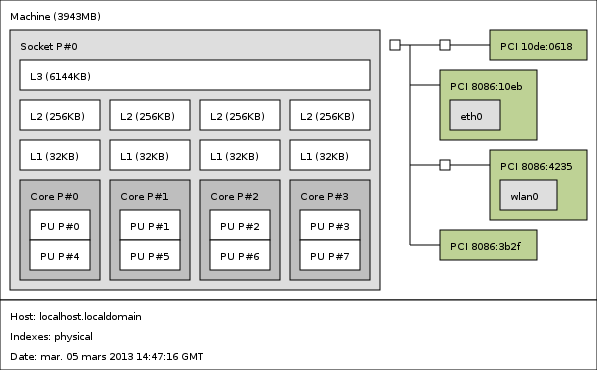
\includegraphics[scale=0.35]{topo.png}
\caption{Topology}
\label{topo}
\end{figure}

\subsection{Software Considerations}

The machine used for this coursework runs a Fedora 18 distribution. This is the exact information:
\begin{lstlisting}
$ uname -a
Linux localhost.localdomain 3.8.1-201.fc18.x86_64 #1 SMP Thu Feb 28 19:23:08 UTC
2013 x86_64 x86_64 x86_64 GNU/Linux
\end{lstlisting}



%-------------------------------------------------------------------------
\section{The Sequential Issue}

\subsection{Analysis}

\subsection{Optimization}


%------------------------------------------------------------------------
\section{CPU Parallelization}

\subsection{Analysis}

\subsection{Optimization}

%-------------------------------------------------------------------------
\section{GPU Acceleration}

\subsection{Analysis}

\subsection{Optimization}


\end{document}